\documentclass[]{beamer}
\usepackage[utf8]{inputenc}
\usepackage[english]{babel}
\usepackage{url}
\usepackage{hyperref}
%\usepackage[usenames,dvipsnames]{color}
\usepackage{units}
\usepackage{verbatim}
\usepackage{listings}
\usepackage{ulem}\normalem
\usepackage[absolute,overlay]{textpos}
\hypersetup{pdfsubject={More than batteries included: NeuroDebian},%
  pdfkeywords={Debian, NeuroDebian, packaging, Python, neuroscience},%
  colorlinks,citecolor=blue,linkcolor=green,urlcolor=blue}


\newcommand{\SWIRLBG}{%
  \usebackgroundtemplate{\includegraphics[width=\paperwidth]{swirl-lightest}}}

\newcommand{\PYMVPABIG}{%
  \usebackgroundtemplate{\\ \\ \\ \includegraphics[width=\paperwidth]{pymvpa_logo_fromfusionposter_tuned/dim}}}

% for footnote references without marks
\long\def\refnote#1{\begingroup\def\thefootnote{\fnsymbol{footnote}}
\footnote[0]{\hspace{-5mm}\footnotesize{#1}}\endgroup}

\graphicspath{
 {../pics/}
 {pics/}
}

% NeuroDebian theme
\mode<presentation>
{
  \usetheme{Boadilla}
  \usecolortheme{beaver}
  \useinnertheme{rectangles}
  \setbeamertemplate{headline}[default]
  \setbeamertemplate{navigation symbols}{}
  \definecolor{debian}{RGB}{215,6,83}
  \definecolor{ndheadline}{RGB}{32,67,92}
  \definecolor{ndmint}{RGB}{238,255,204}
  \definecolor{ndblue}{RGB}{235,243,249}
  \definecolor{nddarkblue}{RGB}{61,123,165}
  \definecolor{ndpink}{RGB}{243,237,240}
  \definecolor{ndyellow}{RGB}{250,242,234}
  \setbeamercolor{alerted text}{fg=debian}
  \setbeamercolor{structure}{fg=debian}
  \setbeamercolor{titlelike}{bg=gray!10!white,fg=debian}
  \setbeamercolor{frametitle}{fg=ndheadline}
  \setbeamercolor{block title}{fg=white,bg=nddarkblue!60!gray}
  \setbeamercolor{block body}{bg=ndblue}
  \setbeamercolor{block title example}{fg=white,bg=green!25!gray}
  \setbeamercolor{block body example}{bg=ndmint}
  \setbeamercolor*{palette primary}{bg=black!10!white,fg=black!30!debian}
  \setbeamercolor*{palette secondary}{fg=white,bg=debian!80!lightgray}
  \setbeamercolor*{palette tertiary}{bg=gray,fg=white}
}

%%% Local Variables: 
%%% mode: latex
%%% TeX-master: t
%%% End: 


\graphicspath{
 {../pics/borrowed}
 {../pics/}
 {pics/}
}

\newcommand{\veil}[0]{%
 \begin{textblock*}{115mm}[0,0](7mm, 20mm)%
    \includegraphics[width=\linewidth,height=0.7\textheight,clip=on]{neuropy_history_tuned/00veil_sw.png}
  \end{textblock*}}

\newcommand{\veilquote}[2]{%
  \veil
  \begin{textblock*}{105mm}[0,0](12mm,20mm)%
    \vspace{5em}
    #1
    \flushright{--#2}
  \end{textblock*}
}

\newcommand{\veilverbatim}[1]{%
  \veil
  \begin{textblock*}{105mm}[0,0](12mm,20mm)%
    \begin{small}
    \begin{verbatim}
#1
    \end{verbatim}
    \end{small}
  \end{textblock*}
}

%\includeonlyframes{}

\title[$\pi$`s in Debian]%
{$\pi$`s in Debian or Scientific Debian:\newline {NumPy}, {SciPy} and beyond
}
\author[Halchenko]{Yaroslav O. Halchenko}
\institute[Debian, Dartmouth]{Debian Project,\newline Dartmouth College, USA}
\date[EuroScipy 2011]{EuroScipy 2011, Paris, France}
%{\tiny May 4th 2011}}

\begin{document}

{\SWIRLBG
\begin{frame}
  \titlepage
\end{frame}
}

\begin{frame}
\thispagestyle{empty}

Scientists report:
\begin{center}
    \includegraphics[width=0.7\textwidth]{neurolinux_paper_mainttime}\\
    {\begin{tiny}
        \refnote{Hanke M and Halchenko YO (2011) \emph{Neuroscience runs on GNU/Linux.}\linebreak
          Front. Neuroinform. 5:8.
          doi: \href{http://www.frontiersin.org/neuroinformatics/10.3389/fninf.2011.00008/full}{10.3389/fninf.2011.00008}}
    \end{tiny}}
\end{center}
\end{frame}

\begin{frame}{Debian: once upon a time}
  \begin{quotation}
    \noindent Fellow Linuxers,\\
    This is just to announce the \uline{imminent completion} of a
    \textbf{brand-new Linux release}, which I'm calling the \textbf{Debian
      Linux Release}.
    [\ldots] \\
    \hfill \alert{Deb}ra's husband \emph{\alert{Ian} A Murdock}, 16/08/1993 \\
    \hfill \texttt{\small comp.os.linux.development} %\\
  \end{quotation}
  \begin{itemize}
  \item \alert{non-commercial} distro, competitive in the OS market
  \item \alert{easy} to install
  \item built \alert{collaboratively} by \uline{volunteer} software \uline{experts}
  \item 1st major distro developed ``\alert{openly} in the spirit of GNU''
  \end{itemize}
\end{frame}

\begin{frame}{Debian: early history \only<2->{of my life}}
  \begin{itemize}
  \item[1993] announcement
  \item[1994] Debian manifesto \vfill
  \item[1997] Debian \alert{Social Contract} with the Free Software community
    \begin{itemize}
    \item 100\% Free Software: Debian Free Software Guidelines
    \item give back
    \item don't hide problems
    \item priorities: users \& Free Software
    \end{itemize} \vfill
  \item[1998] Debian \alert{Constitution} \\
    structure and rules of a Free-Software-compatible democracy
    \begin{itemize}
    \item default: do-cracy, consensus + working code
    \item democracy, when needed
    \item scaffolding: DPL, secretary, etc.
    \end{itemize}
  \item<2->[2000] I use Debian for the first time
  \item<2->[2004] I submit the first bug report\\
    I contribute my first package
  \item<2->[2006] I become an official Debian Developer
  \end{itemize}
\end{frame}

\begin{frame}[t]{Debian\only<1-15>{, 18 years later\only<14>{: 133 \alert{derivatives}}}%
  \only<16>{: the Universal OS}}
  \begin{itemize}
  \item $\approx$ 17'000 source packages
  \item $\approx$ 33'000 binary packages (amd64/sid/main)
  \item largest n.~of \alert{ports} among mainstream distros (11
    official, 4 unofficial)
    \begin{itemize}
    \item 2 non-Linux ports: GNU/kFreeBSD + (unofficial Hurd)
    \end{itemize}\pause
  \item $12$ \alert{stable} releases
    \only<2-6>{%
    \begin{itemize}
    \item The latest stable release:\\
      \flushright{\only<2>{\alert{FUD ALERT:} 5 years ago}\pause 6.0 Squeeze, February 6th 2011}
    \item \pause oldstable [still supported]: 5.0 Lenny, February 14th 2009
    \item \pause old oldstable [February 15th, 2010]: 4.0 Etch, April 2nd 2007
    \end{itemize}
    \begin{itemize}
    \item Released $\approx$ 2 years
    \item Security support for 3 years\pause
    \item Upgradable
    \end{itemize}
  }
  \item<7-> 2 1/2 \alert{rolling} releases: testing, unstable (sid),
    experimental
  \item<11-> 133 ``\alert{derivative}'' distributions\pause
    \hfill {\small (source: \href{http://www.distrowatch.com}{distrowatch.com})}
  \item<15-> $\approx$ 900 active \alert{DDs} + $\approx$200 \alert{DMs} + thousands other
    \alert{contributors}
%  \item \ldots
  \end{itemize}
  \uncover<16->{
  \pause
  \begin{center}\Large
    \includegraphics[width=0.4\textwidth]{borrowed/success_baby}
  \end{center}}

\only<8-10>{\begin{textblock*}{10.5cm}[0,0](11mm,16mm)\fcolorbox{lightgray}{lightgray}{%
\includegraphics[width=\linewidth]{debian_flavors_tuned/stable}}\end{textblock*}}%
\only<8>{\begin{textblock*}{10.5cm}[0,0](10mm,15mm)\fcolorbox{debian}{white}{%
\includegraphics[width=\linewidth]{debian_flavors_tuned/stable}}\end{textblock*}}%
\only<9>{\begin{textblock*}{10.5cm}[0,0](10mm,15mm)\fcolorbox{debian}{white}{%
\includegraphics[width=\linewidth]{debian_flavors_tuned/allsuites}}\end{textblock*}}%
\only<10>{\begin{textblock*}{10.5cm}[0,0](10mm,15mm)\fcolorbox{debian}{white}{%
\includegraphics[width=\linewidth]{debian_flavors_tuned/derivatives}}\end{textblock*}}

% Linuxes tags
\only<12-14>{\begin{textblock*}{10.5cm}[0,0](11mm,16mm)\fcolorbox{white}{white}{%
\includegraphics[width=\linewidth]{linuxes-tagcloud-201108}}\end{textblock*}}%
\only<13>{\begin{textblock*}{10.5cm}[0,0](11mm,16mm)\fcolorbox{white}{white}{%
\includegraphics[width=\linewidth]{linuxes-tagcloud-201108_tuned/02debians+redhats}}\end{textblock*}}%
\only<14>{\begin{textblock*}{10.5cm}[0,0](11mm,16mm)\fcolorbox{white}{white}{%
\includegraphics[width=\linewidth]{linuxes-tagcloud-201108_tuned/00ubudebians}}\end{textblock*}}%

\end{frame}

\begin{frame}{More on Debian \& its derivatives}

\emph{Who the bloody hell cares about Debian?}\\
Stefano Zacchiroli, Debian project leader, LCA 2011, Australia\\
\begin{tiny}\url{http://upsilon.cc/~zack/blog/posts/2011/01/who_the_bloody_hell_cares_about_Debian/}
\end{tiny}

\end{frame}

\section{Debian Community}

\begin{frame}[t]{Debian community: DebConf 2011, 262 humanoids}
$\approx$ 900 active \alert{DDs}, $\approx$200 \alert{DMs}, $>$100 Teams
\begin{center}
\includegraphics[width=\linewidth]{Dc11group_1024}
\end{center}
\end{frame}

\begin{frame}[t]{Debian community: DebConf 2007-2011, $\approx$ 900}
$\approx$ 900 active \alert{DDs}, $\approx$200 \alert{DMs}, $>$100 Teams
\vspace{-0.5em}
\begin{center}
\includegraphics[width=0.49\linewidth]{Dc07group_1024}
\includegraphics[width=0.49\linewidth]{Dc08group_1024}\\
\begin{textblock*}{0.49\linewidth}[0,0](0.1\linewidth, 55mm)%
\includegraphics[width=\linewidth]{Dc09group_1024}
\end{textblock*}
\begin{textblock*}{0.49\linewidth}[0,0](0.53\linewidth, 55mm)%
\includegraphics[width=\linewidth]{Dc10group_1024}\\
\includegraphics[width=\linewidth]{Dc11group_1024}
\end{textblock*}
\end{center}
\end{frame}


\begin{frame}[t]{Debian: the community}
$\approx$ 900 active \alert{DDs}, $\approx$200 \alert{DMs}, $>$100 Teams
\begin{itemize}
\item Thousands of participants
\item \href{http://www.perrier.eu.org/weblog/2011/06/12}{Debian developers from 57 countries}\\
  \alert{Finland: 5,77 DDs / million}
\item Teams:\\
  \url{http://wiki.debian.org/Teams}
\item Internationalization (i10n):\\
  \url{http://www.debian.org/international/l10n/po/rank}

\item Different fields of endeavor:
  \begin{itemize}
  \item \href{http://wiki.debian.org/DebianScience}{Debian Science}
  \item \href{http://www.debian.org/devel/debian-med/index.en.html}{Debian Med}
  \item \href{http://debichem.alioth.debian.org}{Debichem}
  \item \href{http://neuro.debian.net}{NeuroDebian}
  \item \ldots
  \end{itemize}
\end{itemize}
\end{frame}

\begin{frame}{Debian's -ocracies}
  \begin{enumerate}
  \item \alert{do-ocracy}
    \begin{quotation}
      An individual Developer may make any technical or nontechnical decision
      with regard to their own work;\\
      \hfill {\small\normalfont Debian Constitution, §3.3.1.1}
    \end{quotation}
  \item \alert{democracy}
    \begin{quotation}
      Each decision in the Project is made by one or more of the following: \\
      1. The Developers, by way of General Resolution [...] \\
      \hfill {\small\normalfont Debian Constitution, §2}
    \end{quotation}
  \end{enumerate}

  that means:
  \begin{itemize}
  \item reputation follows work, easy to have an impact
  \item no benevolent dictator, no oligarchy
  \item \alert{no imposed decisions} \\
    {\small by who has money, infrastructure, employees, \ldots}
  \end{itemize}
\end{frame}


\section{Python in Debian}


\begin{frame}[fragile]{Pythons in Debian}
  \begin{description}[XXX]
  \item[Python2]:\\
    \begin{itemize}
    \item 2.5 [in stable], 2.6 [default] and 2.7 [testing, sid]
    \item 2630 projects out of 16525 (16\%) use Python(2)\\
      Used by some core tools:\\
      dput, git-buildpackage, piuparts, reportbug, ...
    \item 2.7 as the default in experimental\\
      \url{http://bugs.debian.org/622279}\\
      17 bugs holding the transition\\
      2.7 as the default -- the release goal for wheezy
    \end{itemize}
  \item[Python3]<2->:\\
    \begin{itemize}
    \item 3.1 [in stable], 3.2 [testing, sid]
    \item 65 packages dependent on Python3
    \end{itemize}
  \item[Maintained by]<3->:\\
    \textbf{Matthias Klose}, Piotr Ożarowski, Scott Kitterman, Tollef
    Fog Heen, Raphael Hertzog, Michael Vogt, Marc Deslauriers,
    Colin Watson
  \end{description}
\end{frame}

\begin{frame}[fragile]{Who cares about Python in Debian}
  \begin{description}[XXX]
  \item[111 teams]:\\
      \begin{itemize}
      \item Debian Python Modules Team\\
        \url{https://alioth.debian.org/projects/python-modules}\\
        207 members \\
%        Admins: Gustavo Franco, Guilherme de Siqueira Pastore, Piotr Ożarowski, Bernd Zeimetz \\
        \alert<2>{maintain NumPy and SciPy}\\
      \item Python Applications Packaging Team\\
        \url{https://alioth.debian.org/projects/python-apps}\\
        133 members
      \end{itemize}
  \item[549 individuals]
  \end{description}
\end{frame}

%YOH%\only<2>{\veilverbatim{
%YOH%/usr/share/doc/python-minimal/changelog.Debian.gz \\
%YOH%     51 Matthias Klose  \\
%YOH%     34 Piotr Ożarowski \\
%YOH%     15 Scott Kitterman \\
%YOH%      1 Adeodato Simó
%YOH%}}
%YOH%
%YOH%\only<4>{\veilverbatim{
%YOH%/usr/share/doc/python3-minimal/changelog.Debian.gz \\
%YOH%     21 Piotr Ożarowski \\
%YOH%     13 Matthias Klose  \\
%YOH%      8 Scott Kitterman \\
%YOH%      2 Anders Kaseorg
%YOH%}}

\begin{frame}{$\pi$'s in Debian%
\only<2>{: popcon is growing}%
\only<3>{: \alert{NumPy is on 40\% of Debian boxes}}%
\only<4>{: SciPy is not waiting}%
\only<7>{: the Core}%
\only<8>{: numerical computing}%
\only<9>{: machine/statistical learning}%
\only<10>{: brain sciences}%
\only<11>{: games}%
    }
  \begin{itemize}
  \item<1-5,12-> Popularity Contest\\
    \url{http://popcon.debian.org}\\
    \uncover<5->{\alert{Numpy is on 40\% of Debian installations}}
  \item<5,12-> \emph{apt-cache rdepends python-numpy}
    \begin{itemize}
    \item 158 packages depend on NumPy
    \item 40 packages depend on SciPy
    \end{itemize}
  \item<12-> Cover variety of applications \alert{out-of-the-box}
  \item<12-> Most recent additions [Debian sid]
    \begin{itemize}
    \item FreeNect (Free Kinect driver)
    \item PyCUDA
    \item PyOpenCL
    \item scikits.statsmodels
    \end{itemize}
  \end{itemize}

\only<2-4>{\begin{textblock*}{10.5cm}[0,0](12mm,17mm)\fcolorbox{lightgray}{lightgray}{%
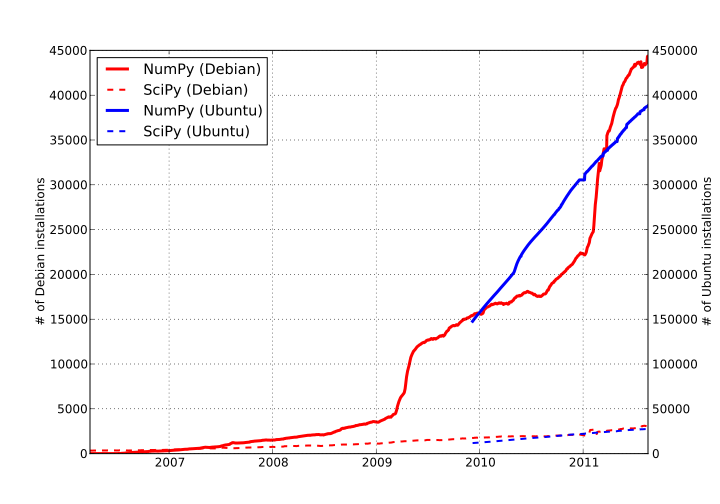
\includegraphics[width=\linewidth]{popcon/pyes_counts}}\end{textblock*}}%
\only<2>{\begin{textblock*}{10.5cm}[0,0](11mm,16mm)\fcolorbox{red}{white}{%
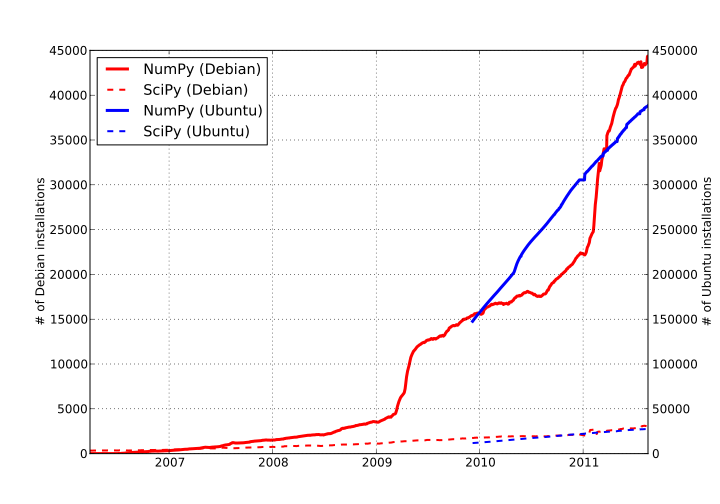
\includegraphics[width=\linewidth]{popcon/pyes_counts}}\end{textblock*}}%
\only<3>{\begin{textblock*}{10.5cm}[0,0](11mm,16mm)\fcolorbox{red}{white}{%
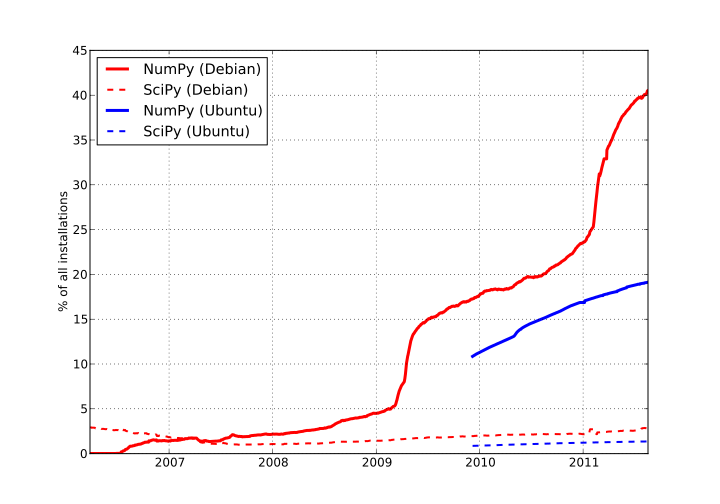
\includegraphics[width=\linewidth]{popcon/pyes_percents}}\end{textblock*}}%
\only<4>{\begin{textblock*}{10.5cm}[0,0](11mm,16mm)\fcolorbox{red}{white}{%
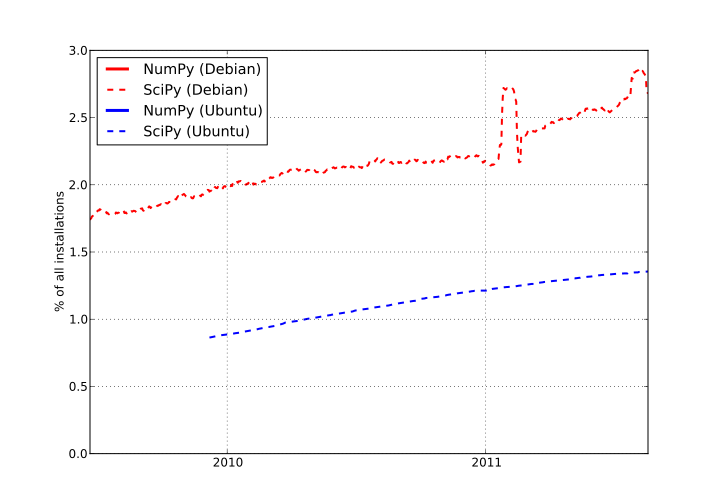
\includegraphics[width=\linewidth]{popcon/pyes_percents_zoom}}\end{textblock*}}%

\only<6>{\begin{textblock*}{10.5cm}[0,0](11mm,16mm)\fcolorbox{white}{white}{%
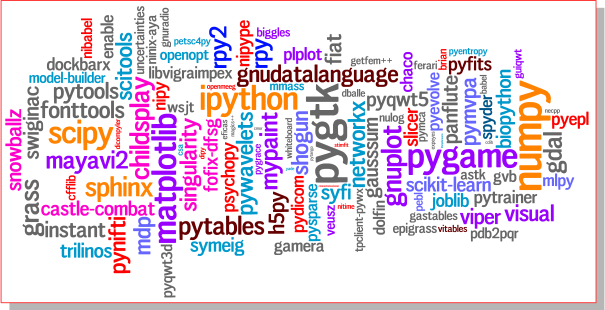
\includegraphics[width=\linewidth]{debian_nipy_kids}}\end{textblock*}}%
\only<7>{\begin{textblock*}{10.5cm}[0,0](11mm,16mm)\fcolorbox{white}{white}{%
\includegraphics[width=\linewidth]{debian_nipy_kids_tuned/core}}\end{textblock*}}%
\only<8>{\begin{textblock*}{10.5cm}[0,0](11mm,16mm)\fcolorbox{white}{white}{%
\includegraphics[width=\linewidth]{debian_nipy_kids_tuned/computing}}\end{textblock*}}%
\only<9>{\begin{textblock*}{10.5cm}[0,0](11mm,16mm)\fcolorbox{white}{white}{%
\includegraphics[width=\linewidth]{debian_nipy_kids_tuned/ml}}\end{textblock*}}%
\only<10>{\begin{textblock*}{10.5cm}[0,0](11mm,16mm)\fcolorbox{white}{white}{%
\includegraphics[width=\linewidth]{debian_nipy_kids_tuned/neuro}}\end{textblock*}}%
\only<11>{\begin{textblock*}{10.5cm}[0,0](11mm,16mm)\fcolorbox{white}{white}{%
\includegraphics[width=\linewidth]{debian_nipy_kids_tuned/games}}\end{textblock*}}%

\only<8>{\refnote{\begin{tiny}\url{http://blends.alioth.debian.org/science/tasks/numericalcomputation}\end{tiny}}}
\only<9>{\refnote{\begin{tiny}\url{http://blends.alioth.debian.org/science/tasks/machine-learning}\end{tiny} }}
\only<10>{\refnote{\url{http://neuro.debian.net}}}
\end{frame}

\begin{frame}{Debian is beneficial for ``Upstream''}
  \begin{block}{}
    Debian provides a robust deployment platform, which helps to ...
  \end{block}
\begin{itemize}
  \item iron out problems
    \begin{itemize}
    \item packaged/tested on the system nearly identical to the others
    \item binary builds across all supported platforms
    \item (optional) package build-time (unit-)testing
    \item "stable" release is stable -- bugs triaged \emph{before} the release
    \end{itemize}
  \item deliver
    \begin{itemize}
    \item 133 derivatives
    \item Mark S.: ``200 millions of Ubuntu users in 3 years and 9 months''
    \item official Debian mirrors in 46 countries \\
      \url{http://www.debian.org/mirror/list}
    \end{itemize}
  \item engage more caring hands
    \begin{itemize}
    \item QA activities: archive rebuilds (FTBFS), package QA tools
    \item centralized transitions
    \end{itemize}
  \item report usage statistics \\
    \url{http://popcon.debian.org}
  \end{itemize}

\only<2>{%
  \veilquote{
    I have always found my friends Debian developers to
    be pretty good at getting me do boring but useful stuff.
  }{Gael Varoquaux}%(mayavi2, joblib, \ldots)}
}

\end{frame}

\begin{frame}{Help yourself to help Debian}
\begin{itemize}
\item Have a \alert{deterministic version}
\item Be conscious about \emph{all} \alert{licenses}
\item Allow for \alert{modularity}
  \begin{itemize}
  \item use (documented) "standard" build mechanisms
  \item treat 3rd party as 3rd party
    \begin{itemize}
    \item no forks -- forward fixes upstream, request bugfix releases
    \item allow an option to build against system-installed versions
    \end{itemize}
  \item be compatible with recent released versions NumPy/SciPy
  \end{itemize}
\item Be prepared for \alert{feedback}
\item Provide unit-/doc- \alert{tests} and examples
  \begin{itemize}
  \item easy way to run only lightweight portion (for build-time testing)
  \item conventional means to run the tests
  \item use tempfile.* instead of the work-tree
  \item do not hardcode matplotlib backends (unless required)
  \end{itemize}
\item Test/use your software on Debian\\
  (especially during Debian freeze)
\end{itemize}

\refnote{\begin{tiny}\url{http://neuro.debian.net/blog/2011/2011-08-23_getting_stuff_packaged.html}\end{tiny} }

\end{frame}

\begin{frame}{Debian is a rich platform for Python development}
  \begin{block}{}
    Debian facilitates software development by providing \alert{out-of-the-box}...
  \end{block}
  \begin{itemize}
  \item Multiple supported versions of Python
  \item Python Editors/IDEs/refactoring tools
    \begin{itemize}
    \item vim, emacs (GNU Python mode, python-mode, ropemacs)
    \item DrPython, Eric, Geany, gEcrit, PIDA, Spyder, ...
    \item pylint, pyflakes
    \item rope, bicyclerepair
    \end{itemize}
  \item debugging facilities
    \begin{itemize}
    \item pdb, pydb, pudb, winpdb
    \item advanced extensions debugging\\
      (in a minute)
    \end{itemize}
  \item easy ways to bootstrap a complete system\\
    (in 2 minutes)
  \end{itemize}
\end{frame}

\def\Maroon{}%\color{Maroon}}
\def\Green{}%\color{Green}}

\begin{frame}{Advanced extensions debugging facilities}
  \begin{description}
  \item[GDB] inspect Python stack
  \item[Valgrind] pin-point segfaults and memory leaks
  \item[Profiling GUI]kcachegrind, hotshot + kcachegrind-converters\\
    \begin{tiny}
      \url{https://github.com/PyMVPA/PyMVPA/blob/master/tools/profile}
    \end{tiny}
  \item[DMTCP] snapshot lengthy computations
  \item[FReD] [coming] reversible debugger
  \end{description}
\end{frame}

\begin{frame}[fragile]{GDB: inspect Python stack}
\begin{verbatim}
> gdb --args /usr/bin/python-dbg segfault.py
GNU gdb (GDB) 7.3.50.20110627-cvs-debian
...
Program received signal SIGSEGV, Segmentation fault.
...
(gdb) py <TAB>
py-bt      py-down    py-list    py-locals  py-print   py-up      python
\end{verbatim}
\end{frame}

\begin{frame}[fragile]{GDB: Python stack}
\begin{verbatim}
(gdb) bt
...
#10  ... /arrayprint.py, line 156, in _leading_trailing ...
#11  ... at ../Python/ceval.c:3836 ...
(gdb) py-bt
#10 Frame 0xf5c6d0, ... /arrayprint.py, line 156 ....
                                     a[-_summaryEdgeItems:]))
#13 Frame 0xf63230, ... ./arrayprint.py, line 162 ...
                min(len(a), _summaryEdgeItems))]
(gdb) py-up
#13 Frame 0xf63230 ...
                min(len(a), _summaryEdgeItems))]
(gdb) py-down
#10 Frame 0xf5c6d0 ...
                          a[-_summaryEdgeItems:]))
\end{verbatim}
\end{frame}

%POST%\begin{frame}[fragile]{GDB: location in Python code}
%POST%\begin{verbatim}
%POST%  (gdb) py-list
%POST% 153  if a.ndim == 1:
%POST% 154      if len(a) > 2*_summaryEdgeItems:
%POST% 155          b = _nc.concatenate((a[:_summaryEdgeItems],
%POST%>156                                   a[-_summaryEdgeItems:]))
%POST% 157      else:
%POST% 158          b = a
%POST% 159  else:
%POST%\end{verbatim}
%POST%\end{frame}
%POST%
%POST%\begin{frame}[fragile]{GDB: Python variables}
%POST%\begin{verbatim}
%POST%(gdb) py-locals
%POST%a = <numpy.ndarray at remote 0xf2db40>
%POST%_nc = <module at remote 0xaa9e30>
%POST%(gdb) py-print _summaryEdgeItems
%POST%global '_summaryEdgeItems' = 3
%POST%(gdb) py-print a
%POST%local 'a' = <numpy.ndarray at remote 0xf2db40>
%POST%\end{verbatim}
%POST%\end{frame}

\begin{frame}[t]{DMTCP: Snapshot your Python}
\begin{block}{Why?}
  \begin{itemize}
  \item Stop/resume the lengthy task
    \begin{itemize}
    \item across power outages
    \item ``reversible'' debugging
    \end{itemize}
  \item Move the task across identical boxes (PBS, Condor)
  \end{itemize}
\end{block}

\only<1>{%
\begin{itemize}
  \item {\Green D}istributed {\Green M}ulti{\Green T}hreaded
	 {\Green C}heck{\Green P}ointing
  \item Works with Linux kernel 2.6.9 and later
  \item Supports sequential and multi-threaded computations
	across single/multiple hosts
  \item Entirely in user space (no kernel modules or root privilege)
  \item Transparent (no recompiling, no re-linking)
  \item DMTCP Team centered around Northeastern~\hbox{U.}, with
	 collaborators from MIT and
	 Siberian State \hbox{U.} of \hbox{Telecom.} and Informatics
  \item Available in Debian $\ge$ wheezy (current testing)
\end{itemize}}

\only<2>{\begin{exampleblock}{STANDALONE USAGE}
{\tt
\hbox{}~~~~dmtcp\_checkpoint a.out \\
\hbox{}~~~~dmtcp\_command --checkpoint \\
\hbox{}~~~~dmtcp\_restart ckpt\_a.out\_*.dmtcp \\
}
\end{exampleblock}}

\only<3>{\begin{exampleblock}{Python interface}
In the next release
\end{exampleblock}}

\only<4>{\begin{exampleblock}{FReD: Fast Reversible Debugger (WiP)}
\begin{center}
{\includegraphics[width=0.6\textwidth]{borrowed/fred-commands}}
\begin{tiny}\url{http://www.cs.wisc.edu/condor/CondorWeek2011/wednesday_condor.html}\end{tiny}
\end{center}
\end{exampleblock}}
\end{frame}


\begin{frame}[fragile]{Bootstrapping a complete Debian system}
\begin{block}{Why?}
  \begin{itemize}
  \item build/test/use previous or upcoming Debian (or Ubuntu) release
  \item get clean environment (track dependencies)
  \item mimic user's setup
  \end{itemize}
\end{block}
\begin{itemize}
\item<2-> debootstrap + schroot: install into any directory
\item<2-> vmdebootstrap: generate a virtual machine\\
  \url{http://blog.liw.fi/posts/vmdebootstrap/}
\item<2-> Fully Automated Installation (FAI): \url{http://fai-project.org/}
\item<2-> VirtualBox: install or use pre-crafted virtual appliance
\item<2-> Cloud: \url{http://wiki.debian.org/Cloud}
\end{itemize}
\end{frame}

\begin{frame}[fragile]{debootstrap + schroot}
\begin{verbatim}
> debootstrap sid /var/cache/chroots/sid-amd64
> sudo bash -c "cat << EOF >| /etc/schroot/chroot.d/sid-amd64
[sid-amd64]
description=Debian sid (forever unstable) [amd64]
type=directory
location=/var/cache/chroots/sid-amd64
users=YOURLOGIN
aliases=unstable,sid,default
EOF"
> schroot
\end{verbatim}
\end{frame}

\begin{frame}{NeuroDebian VM in VirtualBox}
  \begin{center}
    \includegraphics[width=\linewidth]{ndshot-vm-osx+psychopy}\\
  \url{http://neuro.debian.net/vm.html}
\end{center}
\end{frame}


\begin{frame}{Ways to contribute}

\begin{small}
\url{http://wiki.debian.org/ProjectNews/HowToContribute}\\
\url{http://raphaelhertzog.com/2011/06/30}
\end{small}

\begin{itemize}
\item reportbug (+ patches)
\item Internationalization (i18n): \url{http://www.debian.org/doc/manuals/intro-i18n}
\item packaging
  \begin{itemize}
  \item Luca's tutorial\\
    \emph{apt-get install packaging-tutorial} \\
    \begin{small}\url{http://www.lucas-nussbaum.net/blog/?p=640}\end{small}
  \item Bootstrap packaging of Python modules:\\
    \emph{py2dsc} (python-stdeb package)
  \item Good night reading: \href{http://www.debian.org/doc/debian-policy/}{Debian Policy}
  \item Seek mentor/sponsor-ship: \url{http://mentor.debian.org}
  \item Become ``Debian Maintainer'': \url{http://wiki.debian.org/DebianMaintainer}
  \item Become ``Debian Developer'': \url{http://wiki.debian.org/DebianDeveloper}
  \end{itemize}
\end{itemize}
\end{frame}

% YOH%
%YOH%\only<3>{%
%YOH%\vspace{-3em}
%YOH%{\tt > vmdebootstrap squeeze foo.img http://cdn.debian.net/debian}}
%YOH%
%YOH%\only<5>{
%YOH%\begin{textblock*}{10.5cm}[0,0](11mm,16mm)\fcolorbox{lightgray}{lightgray}{%
%YOH%\includegraphics[width=\linewidth]{ndshot-vm-osx+psychopy}}\\
%YOH%\url{http://neuro.debian.net/vm.html}
%YOH%\end{textblock*}}
%YOH%

\begin{frame}
\includegraphics[width=\textwidth]{borrowed/lolcats/funny-pictures-cat-downloads-brain-chess-sweatshirt.png}
\end{frame}

{\SWIRLBG
\begin{frame}{Acknowledgements}
  \begin{columns}
    \begin{column}{4cm}
      \begin{center}
      \textbf{Michael Hanke}\\
      \end{center}
    \end{column}
    \begin{column}{4cm}
      \begin{center}
      Free and opensource software developers\\
      \vspace{1mm}
      Debian Community
      Python/NumPy/Scipy Maintainers
      \end{center}
    \end{column}
    \begin{column}{4cm}
      \begin{center}
      Jim Haxby
      \end{center}
    \end{column}
  \end{columns}
  \vfill
  \begin{center}
    \vfill
    {\LARGE Thanks!}
    \vfill
    Yaroslav O. Halchenko \\
    \url{yoh@debian.org} \\
    \url{http://www.onerussian.com}
  \end{center}
  {\tiny
    \begin{center}
      \begin{tabular}{l@{\hspace{1em}}l}
        \multicolumn{2}{l}{about the slides:} \\
        available at
        & \url{http://neuro.debian.net/\#publications}
        \\
        \copyright ~ 2011 & Yaroslav O. Halchenko,\\
        portions are:&\\
        \copyright ~ 2010& Stefano Zacchiroli \\
        \copyright ~ 2011& Michael Hanke \\
        slide style & inspired by Stefano Zacchiroli \\
        & \href{http://creativecommons.org/licenses/by-sa/3.0/}{CC BY-SA 3.0 ---
          Creative Commons Attribution-ShareAlike 3.0} \\
      \end{tabular}
    \end{center}}
\end{frame}

%\end{frame}

\begin{frame}[fragile]{How many care about Python}
\begin{verbatim}
> grep-dctrl -s Maintainer -F Build-Depends python
    -o -F Build-Depends python-dev
	-o -F Build-Depends python-all
	/var/lib/apt/lists/*\_sid\_main\_source\_Sources
  | sort | uniq -c | sort -n -r
  | wc -l
660
\end{verbatim}
\end{frame}

\begin{frame}[fragile]{Who cares: teams}
\begin{verbatim}
> grep-dctrl -s Maintainer -F Build-Depends python
    -o -F Build-Depends python-dev
	-o -F Build-Depends python-all
	/var/lib/apt/lists/*\_sid\_main\_source\_Sources
  | sort | uniq -c | sort -n -r
  | grep -e alioth -e team -e Maintainers -e Debian
  | wc -l
111
\end{verbatim}
\end{frame}

\begin{frame}[fragile]{Who cares: teams}
\begin{verbatim}
> ...
  | grep -e alioth -e team -e Maintainers -e Debian | head
    232 Maintainer: Debian Python Modules Team <python-mod...
     57 Maintainer: Debian Tryton Maintainers <tryton@list...
     51 Maintainer: Debian OLPC <debian-olpc-devel@lists.a...
     45 Maintainer: Python Applications Packaging Team <py...
     40 Maintainer: Debian/Ubuntu Zope Team <pkg-zope-deve...
     40 Maintainer: Debian Multimedia Maintainers <pkg-mul...
     26 Maintainer: NeuroDebian Team <team@neuro.debian.ne...
     26 Maintainer: Debian Science Maintainers <debian-sci...
     26 Maintainer: Debian QA Group <packages@qa.debian.or...
     26 Maintainer: Debian Bazaar Maintainers <pkg-bazaar-...
\end{verbatim}
\end{frame}

\begin{frame}[fragile]{Who cares: individuals}
\begin{verbatim}
> grep-dctrl -s Maintainer -F Build-Depends python
    -o -F Build-Depends python-dev
	-o -F Build-Depends python-all
	/var/lib/apt/lists/*\_sid\_main\_source\_Sources
  | sort | uniq -c | sort -n -r
  | grep -v -e alioth -e team -e Maintainers -e Debian
  | wc -l
549
\end{verbatim}
\end{frame}

\begin{frame}[fragile]{Who cares: individuals}
\begin{verbatim}
> ...
  | head
26 Maintainer: Matthias Klose <doko@debian.org>
16 Maintainer: David Paleino <dapal@debian.org>
14 Maintainer: Arnaud Fontaine <arnau@debian.org>
13 Maintainer: Jelmer Vernooij <jelmer@debian.org>
12 Maintainer: Pierre Chifflier <pollux@debian.org>
12 Maintainer: Josselin Mouette <joss@debian.org>
11 Maintainer: Georges Khaznadar <georgesk@ofset.org>
11 Maintainer: Chris Lamb <lamby@debian.org>
11 Maintainer: Alessio Treglia <alessio@debian.org>
10 Maintainer: Scott Kitterman <scott@kitterman.com>
\end{verbatim}
\end{frame}

\begin{frame}[fragile]{NumPy: who cared}
\begin{verbatim}
/usr/share/doc/python-numpy/changelog.Debian.gz
     22 Marco Presi (Zufus)
     20 Ondrej Certik
     13 Kumar Appaiah
      9 Sandro Tosi
      9 Matthias Klose
      2 Tiziano Zito
      ... 15 more ...
\end{verbatim}
\end{frame}

\begin{frame}[fragile]{SciPy: who cared}
\begin{verbatim}
/usr/share/doc/python-scipy/changelog.Debian.gz
     15 Marco Presi (Zufus)
     14 Ondrej Certik
      7 José Fonseca
      7 Alexandre Fayolle
      5 Luca Falavigna
      4 Sandro Tosi
      3 Varun Hiremath
      3 Piotr Ożarowski
      2 Matthias Klose
      ... 5 more ...
\end{verbatim}
\end{frame}


\begin{frame}{XXX How does Python-software benefit from Debian?}
  \begin{itemize}
    \item<1-> Extended reach
      \begin{itemize}
        \item one \uline{stable} release, two rolling ``release'' flavors
        \item $\approx$120 derivative distributions (distrowatch.org)
      \end{itemize}
    \item<5-> Mutual awareness
      \begin{itemize}
        \item Explicitly documented dependencies
        \item Synchronized transitions
      \end{itemize}
    \item<6-> Less maintenance work through modularity
      \begin{itemize}
        \item 3rd-party software in dedicated packages maintained by someone else
      \end{itemize}
    \item<7-> Continuous integration testing
      \begin{itemize}
        \item 13 hardware architectures
        \item Three kernels
        \item Continuous automated testing for
          \begin{itemize}
            \item Build success
            \item Clean installation/de-installation, Availability of dependencies
            \item Policy compliance
            \item Package conflicts
          \end{itemize}
      \end{itemize}
  \end{itemize}
\end{frame}


\end{document}

%%% Local Variables:
%%% mode: latex
%%% TeX-PDF-mode: t
%%% TeX-master: t
%%% ispell-local-dictionary: "american"
%%% auto-fill-inhibit-regexp: ".*[&|].*[&|].*"
%%% End:
